% !TEX TS-program = pdflatexmk
\documentclass[12pt]{amsart}

%\usepackage[parfill]{parskip}    % Activate to begin paragraphs with an empty line rather than an indent

\usepackage[margin=1in]{geometry}

\usepackage{amsmath,amssymb,amsthm,latexsym,graphicx}
\usepackage[normalem]{ulem}
\usepackage{setspace} %used for doublespacing, etc.
\usepackage{hyperref}
\usepackage{listings}
\usepackage[dvipsnames,usenames]{color}
\usepackage{fancyhdr}
\pagestyle{fancy}
	\renewcommand{\headrulewidth}{0.5pt} % and the line
	\headsep=1cm
	
\DeclareGraphicsRule{.tif}{png}{.png}{`convert #1 `dirname #1`/`basename #1 .tif`.png}

%Some useful environments.
\newtheorem{theorem}{Theorem}
\newtheorem{corollary}[theorem]{Corollary}
\newtheorem{conjecture}[theorem]{Conjecture}
\newtheorem{lemma}[theorem]{Lemma}
\newtheorem{proposition}[theorem]{Proposition}
\newtheorem{definition}[theorem]{Definition}
\newtheorem{example}[theorem]{Example}
\newtheorem{axiom}{Axiom}
\theoremstyle{remark}
\newtheorem{remark}{Remark}
\newtheorem*{exercise}{Exercise}%[section]

%Some shortcuts helpful for our assignments
\newcommand{\bx}{\begin{exercise}}
\newcommand{\ex}{\end{exercise}}

%Some useful shortcuts for our favorite sets of numbers.
%Note, you can use these WITHOUT entering math mode
\def\RR{\ensuremath{\mathbb R}} 
\def\NN{\ensuremath{\mathbb N}}
\def\ZZ{\ensuremath{\mathbb Z}}
\def\QQ{{\ensuremath\mathbb Q}}
\def\CC{\ensuremath{\mathbb C}}
\def\EE{{\ensuremath\mathbb E}}

%Some useful shortcuts for formatting lists
\newcommand{\bc}{\begin{center}}
\newcommand{\ec}{\end{center}}
\newcommand{\be}{\begin{enumerate}}
\newcommand{\ee}{\end{enumerate}}
\newcommand{\bi}{\begin{itemize}}
\newcommand{\ei}{\end{itemize}}

%Some useful shortcuts for formatting mathematical symbols
\newcommand{\ol}[1]{\overline{#1}}
\newcommand{\oimp}[1]{\overset{#1}{\iff}} %labeled iff symbol
\newcommand{\bv}[1]{\ensuremath{ \vec{\mathbf{#1}}} } %makes a vector.
\newcommand{\mc}[1]{\ensuremath{\mathcal{#1}}} %put something in caligraphic font
\newcommand{\normale}{\trianglelefteq}
\newcommand{\normal}{\triangleleft}

%Code for formatting the proofs a little nicer for submitted homework
\makeatletter
\renewenvironment{proof}[1][\proofname]{\par\doublespacing
  \pushQED{\qed}%
  \normalfont \topsep6\p@\@plus6\p@\relax
  \list{}{%
    \settowidth{\leftmargin}{\itshape\proofname:\hskip\labelsep}%
    \setlength{\labelwidth}{0pt}%
    \setlength{\itemindent}{-\leftmargin}%
  }%
  \item[\hskip\labelsep\itshape#1\@addpunct{:}]\ignorespaces
}{%
  \popQED\endlist\@endpefalse
  \singlespacing
}
\makeatother


%Commenting tools for the professor
\newcommand{\mpg}[1]{\marginpar{ #1}} %to put comments in margins
\usepackage{soul}
\definecolor{highlight}{rgb}{1,0.6,0.6}
\sethlcolor{highlight}
\newcommand{\hlm}[1]{\colorbox{highlight}{$\displaystyle #1$}}
\newtheoremstyle{mycomment}{\topsep}{-0in}{\small \itshape \sffamily}{}{\small \itshape\sffamily}{:}{.5em}{}
\theoremstyle{mycomment}
\newtheorem*{acomment}{\color{BrickRed}{Comment}}
\newcommand{\com}[1]{{\color{OliveGreen}\begin{acomment}{#1} %#2 \color{black} 
\end{acomment}\noindent}}
\newcommand{\red}[1]{{\color{BrickRed} #1}}
\newcommand{\blue}[1]{{\color{MidnightBlue}#1}}
\newcommand{\green}[1]{{\color{OliveGreen}#1}}
\newcommand{\mwrong}[2]{\red{\cancel{#1}}\green{#2}}
\newcommand{\wrong}[2]{\red{\sout{#1}}\green{#2}}
\definecolor{OliveGreen}{rgb}{.3,.5,.2}
\definecolor{MidnightBlue}{rgb}{.3,.4,.6}
\newcommand{\pts}[1]{\hfill\blue{{#1}/5}}

\begin{document}
\title{\Large Probability Lab 2}
\author{Christopher Munoz}
\maketitle
\begin{center}
\textbf{Introduction}
\end{center}

\begin{center}
	In this laboratory we are tasked with investigating the nature of games of chance, in particular games involving dice and coin flips. We are tasked with using R in our investigation. 
\end{center}


\vspace{1cm}

\begin{center}
	\textbf{Problem 1}
\end{center}
In this problem, we will explore the sum of the roll of five(the sheet had an error) dice for sample sizes n = 10, 25, 50, 100.

\begin{exercise}[a]
Suppose we roll the five dice and sum the outcomes repeatedly. In this game we earn \$0.25 times this
	sum, for instance, a roll of 1,1,1,1,2 earns \$1.50. We want to find the expected earnings on average of this game. Let $E(Y)$ represent our expected earnings and $E(D)$ represent our expected value for the roll of 1 die. For 5 dice rolls our expected earnings is
	\begin{align*}
		E(D) &= \sum_{k=1}^{6} \frac{k}{6} = \frac{1}{6} + \frac{2}{6} + \frac{3}{6} + \frac{4}{6} + \frac{5}{6} + \frac{6}{6} = \frac{21}{6} = 3.5 \\
		E(Y) &= (1)0.25 * 5 * E(D) \\
		     &= (1)0.25 * 5 * 3.5 \\
		     &= 4.375 \\
	\end{align*}
	So we are expected to earn $ \$4.375$ dollars in a game where we roll 5 die
	For a general case, the function for our expected earnings is $$E(Y) = 0.25 * n * 5 * 3.5$$ Where $n \in \NN$ is the number of games.
\end{exercise}
\begin{exercise}[b]
We simulate rolling 5 dice repeatedly for $n = 10, 25, 50, 100$ games
For each game, we sum the five dice and multiply by $\$0.25$ to get earnings
We plot histograms showing the distribution of earnings
We compare the simulated mean to our theoretical expected value of $\$4.375$
\\ \\ \\ \\ \\
\begin{figure}[h!]
\centering
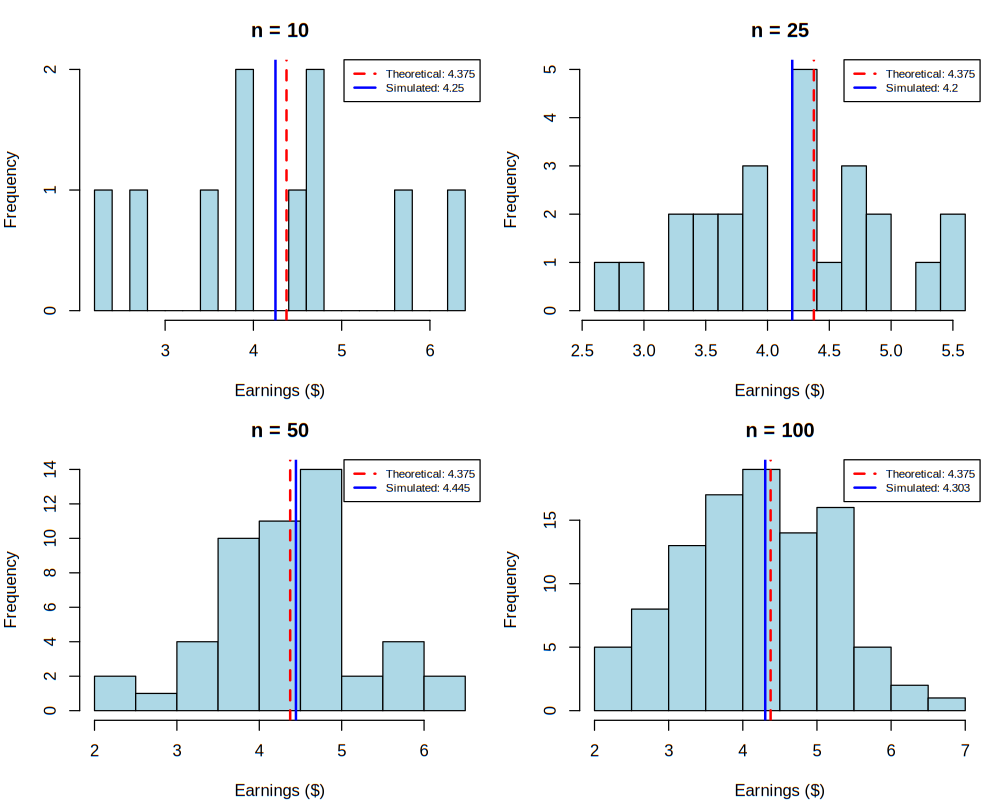
\includegraphics[width=0.95\textwidth]{figures/problem1b.png}
\caption{Distribution of earnings from rolling 5 dice for different sample sizes. The red dashed line shows the theoretical expected value (\$4.375), while the blue solid line shows the simulated mean for each sample size.} We can expect our simulated to converge to our theoretical outcome.
\label{fig:problem1b}
\end{figure}

\end{exercise}

\begin{exercise}[c]
Suppose now that there are three white dice and two blue dice. (Alternatively, we throw the last two
dice separately from the first three.) In this version of the game we earn \$0.30 times the sum of the three
white dice, and you lose \$0.50 for the sum of the two blue dice. For instance, if the white dice come up 2,
1, 4, and the blue diec 2, 3, then we earn \$0.30*(2+1+4) - \$0.50*(2+3) = -\$0.40, or lose 40 cents. We may model this problem as
$$Y = 0.30W - 0.50B$$
where $W$ is the sum of the three white dice and $B$ is the sum of the two blue dice. The expected value is:
\begin{align*}
E(Y) &= 0.30 \cdot E(W) - 0.50 \cdot E(B) \\
E(W) &= 3 \cdot E(D) = 3 \cdot 3.5 = 10.5 \\
E(B) &= 2 \cdot E(D) = 2 \cdot 3.5 = 7 \\
E(Y) &= 0.30(10.5) - 0.50(7) \\
     &= 3.15 - 3.50 \\
     &= -0.35
\end{align*}
So we can expect to lose \$0.35 on average in this game.
\end{exercise}
\begin{center}
	\textbf{Problem 2}
\end{center}
\begin{exercise}
We toss a biased coin repeatedly, with the probability of heads, P (H) = p, for some unknown value
of p. Our goal is to give the best estimate of p that we can. To that end, suppose we flip this coin three
times and that we earn \$5 for each H that comes up, and lose \$3 for each T that comes up.
We were given 3 data sets. They are called earningsN where N = 10, 100, 1000.

Let $k$ be the number of heads in 3 flips and $E$ be our earnings. Note that $k \sim \text{Binomial}(3, p)$ so $E(k) = 3p$. Then:
\begin{align*}
	E &= 5k - 3(3-k) = 5k - 9 + 3k = 8k - 9\\
	E(E) &= 8 \cdot E(k) - 9\\
			 &= 8(3p) - 9\\
			 &= 24p - 9
\end{align*}
Now we can solve for $p$ to get our probability: $$p = \frac{E(E) + 9}{24}$$

We estimate $p$ by using the sample mean earnings as an estimate for $E(E)$:
$$\hat{p} = \frac{\overline{E}+ 9}{24}$$
Now we use our dataset to predict our probability(code is at the end of this document).
\textbf{Results from the Three Datasets:}
\begin{itemize}
\item From \texttt{earnings10} ($n=10$): $\hat{p} = 0.2333$
\item From \texttt{earnings100} ($n=100$): $\hat{p} = 0.3733$
\item From \texttt{earnings1000} ($n=1000$): $\hat{p} = 0.3043$ \\ \\ \\ \\ \\ \\ \\ 
\end{itemize}
\begin{figure}[h!]
\centering
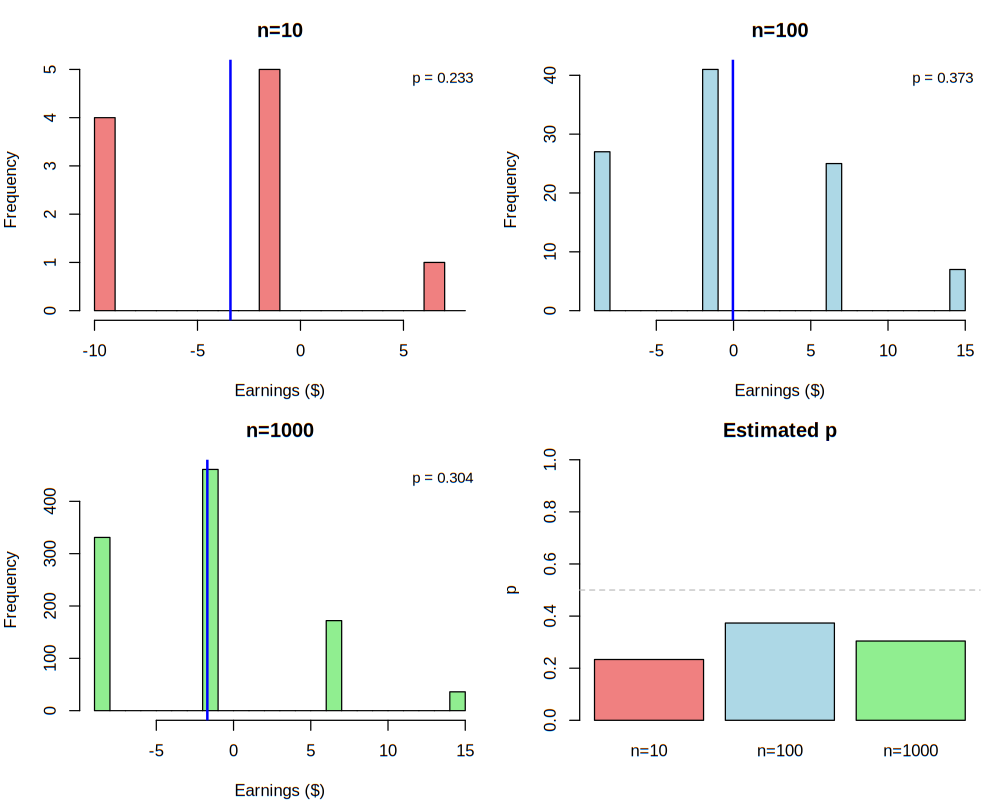
\includegraphics[width=0.95\textwidth]{figures/problem2.png}
\caption{Distribution of earnings and estimated probabilities. The top three panels show earnings distributions for different sample sizes, with blue lines indicating the mean. The bottom-right panel compares the estimated $p$ values across all three datasets.}
\label{fig:problem2}
\end{figure} 
\end{exercise}
I estimate the value of $p$ to be \textbf{0.3043} because the dataset with $n=1000$ provides the most reliable estimate with a larger sample size, the sample mean is a better estimator of the true expected value, reducing the standard error of our estimate. Notice that the estimates from smaller samples ($n=10$ gives $0.2333$ and $n=100$ gives $0.3733$) show more variability, while the $n=1000$ dataset provides a more stable and trustworthy estimate. Therefore, our best estimate is that the biased coin has approximately a 30.43\% probability of landing heads.

\begin{center}
	\textbf{R code for Problem 1}
\end{center}
\begin{lstlisting}
if (!dir.exists("figures")) dir.create("figures")

sample_sizes <- c(10, 25, 50, 100)

simulate_earnings <- function(n) {
  0.25 * rowSums(matrix(sample(1:6, 5*n, replace=TRUE), ncol=5))
}

theoretical_ev <- 4.375

png("figures/problem1b.png", width=1000, height=800, res=120)
par(mfrow=c(2,2), mar=c(4,4,3,1))
for(n in sample_sizes) {
  earnings <- simulate_earnings(n)
  hist(earnings, main=paste("n =", n), xlab="Earnings ($)", col="lightblue", breaks=15)
  abline(v=theoretical_ev, col="red", lwd=2, lty=2)
  abline(v=mean(earnings), col="blue", lwd=2)
  legend("topright", c(paste("Theoretical:", theoretical_ev), paste("Simulated:", round(mean(earnings), 3))), 
         col=c("red", "blue"), lty=c(2, 1), lwd=2, cex=0.7)
  cat("1b: n =", n, "Mean = $", round(mean(earnings), 4), "\n")
}
dev.off()

\end{lstlisting}
\begin{center}
	\textbf{R code for Problem 2}
\end{center}
\begin{lstlisting}
	load("earnings10.dat")
load("earnings100.dat")
load("earnings1000.dat")

estimate_p <- function(earnings, n) {
  p <- (mean(earnings) + 9) / 24
  cat("Problem 2: n =", n, "p =", round(p, 4), "\n")
  p
}

p10 <- estimate_p(earnings10, 10)
p100 <- estimate_p(earnings100, 100)
p1000 <- estimate_p(earnings1000, 1000)

png("figures/problem2.png", width=1000, height=800, res=120)
par(mfrow=c(2,2), mar=c(4,4,3,1))
hist(earnings10, main="n=10", xlab="Earnings ($)", col="lightcoral", 
     breaks=seq(min(earnings10)-1, max(earnings10)+1, by=1))
abline(v=mean(earnings10), col="blue", lwd=2)
legend("topright", paste("p =", round(p10, 3)), cex=0.9, bty="n")

hist(earnings100, main="n=100", xlab="Earnings ($)", col="lightblue", breaks=20)
abline(v=mean(earnings100), col="blue", lwd=2)
legend("topright", paste("p =", round(p100, 3)), cex=0.9, bty="n")

hist(earnings1000, main="n=1000", xlab="Earnings ($)", col="lightgreen", breaks=30)
abline(v=mean(earnings1000), col="blue", lwd=2)
legend("topright", paste("p =", round(p1000, 3)), cex=0.9, bty="n")

barplot(c(p10, p100, p1000), names.arg=c("n=10", "n=100", "n=1000"),
        main="Estimated p", ylab="p", col=c("lightcoral", "lightblue", "lightgreen"), ylim=c(0, 1))
abline(h=0.5, col="gray", lty=2)
dev.off()

cat("\nBest estimate: p =", round(p1000, 4), "\n")

\end{lstlisting}

\end{document}

